%!TEX root = ../template.tex
%%%%%%%%%%%%%%%%%%%%%%%%%%%%%%%%%%%%%%%%%%%%%%%%%%%%%%%%%%%%%%%%%%%%
%% chapter5.tex
%% NOVA thesis document file
%%
%% Chapter with lots of dummy text
%%%%%%%%%%%%%%%%%%%%%%%%%%%%%%%%%%%%%%%%%%%%%%%%%%%%%%%%%%%%%%%%%%%%

\typeout{NT FILE chapter5.tex}%

\chapter{Evaluation}
\label{cha:evaluation}

In order to assess the developed system and answer the Research Questions proposed on Section~\ref{sec:objectives-and-researh-questions},
a user study was conducted. This chapter presents the design and results of this user study, exploring the findings and conclusions on 
the impact of the developed portal variants on usability, naturalness and spatial understanding.

\todo{add summary paragraph}

\section{Protocol}
\label{sec:protocol}

To ensure the validity of the results, the user study was always conducted in the same room, with an available tracking space of 
approximately 2.5m x 2.5m, providing conditions comparable to those available to most common \gls{VR} users~\cite{}. In addition, 
the same hardware was used across all participants to ensure consistency, being composed of: an \textit{Oculus Quest 3} \glsfirst{HMD} and 
a computer equipped with an NVIDIA GeForce RTX 3070 graphics card, 16 GB of RAM and an Intel Core i5-9600K CPU.

Each participant experienced the four portal 
techniques—Traditional Portals, Movable Portals, Interactive Doors, and Revolving Doors—while performing the same tasks within 
the same \glsfirst{VE}. The only variation between participants was the order in which the portal techniques were presented, which 
followed a Latin Square design to minimize bias.

\subsection{Procedure}
\label{sec:procedure}

The experimental session commenced by asking the participant to read the informed consent presented in \todo{add appendix}. After reading, 
agreeing and signing the consent form, users were asked to fill a pre-session Virtual Reality Sickness Questionnaire (VRSQ), available in 
\todo{Add VRSQ annex}. Finally, before starting the session, participants also filled a characterization questionnaire that collected 
information about age, gender, education, experience in VR and video games, and sight problems.

After filling these initial forms, the experiment started with a brief of the context and instructions needed for the study given by the 
researcher. The participant was instructed on how to walk around the environment, how to use their virtual hands and 
information regarding the tasks they were asked to perform.  With the instructions provided, the participant started wearing the 
\gls{HMD} and was free explore to explore the \gls{VE} and complete the aforementioned tasks.

The \gls{VE} depicted a museum, structured in four thematic sections, each composed of four rooms populated with exhibition items. Every 
exhibit included an associated quiz and curious fact, designed to encourage engagement and support spatial memory. Each section differed 
from the others by theme, visual appearance, and the portal technique used to connect the rooms. Additionally, the starting room of each 
section featured a uniquely colored floor to help participants reorient themselves when asked to return to the starting point 
(Figure~\ref{fig:layout}).

\begin{figure}[t]
\centering
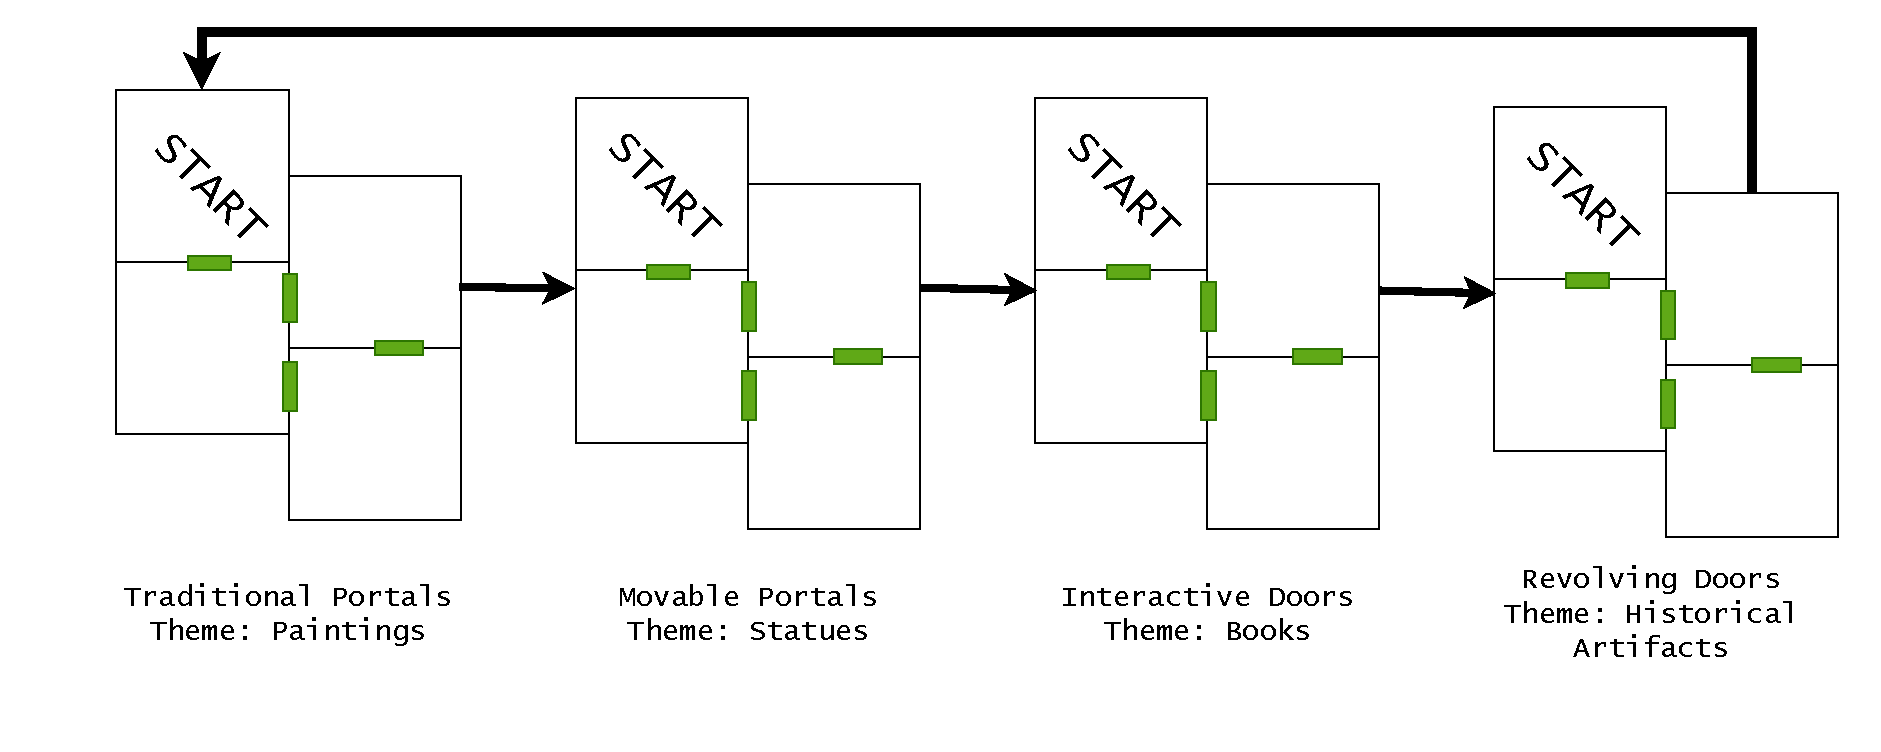
\includegraphics[width=\linewidth]{NOVAthesisFiles/Images/schemes/layout-study.drawio.pdf}
\caption{Layout of the \gls{VE} of the user study.}
\label{fig:layout}
\end{figure}

Within each section, participants completed three tasks in sequence:  
\textbf{1.Exploration Task:} The user freely explored the rooms using the section's associated portal technique, aiming to see and respond 
to every exposition items' quiz. After exploring the whole section, the user was asked to return to the starting room.  
\textbf{2.Spatial Memory Task:} The user was then prompted to point toward an object located in a previously visited room from the starting room. 
To reduce memory bias, participants were allowed to revisit the object before returning to the designated location.  
\textbf{3.Subjective Evaluation:} Finally, the user answered two Likert-scale questions (7-point scale) assessing naturalness and ease 
of use. These questions were presented and answered inside the \gls{VE} to avoid breaks in presence.  

Throughout the session, the experimenter observed and recorded notable behaviors such as hesitations, verbal cues (e.g., “How do I...”), 
or repeated attempts to interact with portals, as objective indicators of usability.  

After completing all four sections, participants removed the \gls{HMD} and filled a post-session questionnaire. This included a post-session 
Virtual Reality Sickness Questionnaire (VRSQ), am Igroup Presence Questionnaire (IPQ), an Immersive Experience Questionnaire (IEQ), 
additional Likert-scale items assessing overall usability, a ranking of the four portal techniques by preference, open-ended questions on perceived 
strengths and weaknesses, and demographic data. Each session lasted approximately 30-45 minutes, depending on the participant's exploration speed.


\subsection{Data Collection}
\label{sec:data}

As mentioned, several methods of quantitative and qualitative data were retrieved from this experiment throughout the procedure.  
For clarity, the collected data are grouped into the following categories:

\textbf{Usability and Naturalness}: To assess subjective user experience, participants rated their agreement with two statements on a 7-point Likert scale (1=Strongly Disagree, 7=Strongly Agree): (1) “I found the transition between rooms natural” and (2) “I found the transition between rooms intuitive / easy to use". To supplement subjective ratings, we captured an objective usability metric by logging usability hesitations. These were defined as any significant pause, verbal expression of confusion, or repeated, incorrect interaction attempts observed by the experimenter.

\textbf{Spatial Understanding}: This was quantified through a pointing task where participants indicated the direction of a target object in a previously visited room. The primary metric was the absolute pointing error, measured in degrees.

\textbf{Presence and Immersion}: The overall sense of being "in" the virtual environment was measured using two standard validated questionnaires: the Igroup Presence Questionnaire (IPQ) and the Immersive Experience Questionnaire (IEQ).

\textbf{Cybersickness}: To monitor for potential adverse effects, participants completed the Virtual Reality Sickness Questionnaire (VRSQ) both before (pre-exposure) and immediately after (post-exposure) the experiment.

\textbf{User Preference and Qualitative Feedback}: Finally, we captured overall user preference by asking participants to order the four portal techniques from 1 (most preferred) to 4 (least preferred). To understand the context behind these rankings and other ratings, the post-session questionnaire included open-ended questions prompting participants to describe the perceived strengths and weaknesses of each portal.

%\section{Tasks}
%\label{sec:tasks}

%\subsection{Rooms}
%\label{sec:rooms}

%\subsection{Exposition Items}
%\label{sec:expo-items}

%\subsection{Pointing Task}
%\label{sec:pointing-task}

%\subsection{Usability Questionnaire}
%\label{sec:questionnaire}


\section{Results}
\label{sec:results}

The results and insights from the user study are presented in this section. After presenting the demographic data of the participants who 
took part in this user study, the collected data aforementioned in the previous section is presented. Finally, a discussion of the 
results is presented, addressing the Research Questions proposed in Section~\ref{sec:objectives-and-researh-questions}.

\subsection{Demographics}
\label{sec:demographics}

We analyzed the data from 31 participants (19 male, 11 female, 1 non-binary), with an average age of 22.5 years (SD = 1.75, range 22-28). In terms of educational backgrounds, 64.5\% of participants held a Bachelor's degree, 29\% held a Master’s degree and 6.5\% reported having High School education or equivalent.

Regarding prior experience with \gls{VR}, 3.2\% of participants reported using \gls{VR} frequently(weekly or more), 3.2\% use \gls{VR} monthly, 29\% used \gls{VR} a few times a year, 38.7\% reported using \gls{VR} once or twice and 25.8\% had never used \gls{VR} before.

In terms of playing video-games, 22.6\% of participants reported playing games frequently(daily), 16.1\% play them weekly, 35.5\% play them monthly, 19.4\% reported playing them a few times a year and 6.5\% don't play video-games.

When asked to rate their perceived sense of orientation/direction on a scale of 1 to 5, 35.5\% of participants rated themselves as 4 and another 35.5\% as 3, so most answers clustered on these values. Following this, 12.9\% of participants rated themselves as 5, another 12.9\% as 2 and 3,2\% as 1.

\todo{Isto se calhar ficava melhor numa tabela}

\subsection{Spatial Understanding}

At the end of each section, users were tasked to point in their perceived direction of a target object in a previously visited room, 
in order to assess users' spatial perception. The primary metric was the absolute pointing error between the answer provided by the 
participant and the preview-based position of the target object, measured in degrees.

A Shapiro-Wilk test showed the data were not normally distributed (p $<$ .05), thus justifying the use of the non-parametric 
Friedman test. Our analysis revealed a highly significant difference in pointing error across the four portal conditions, 
$\chi$²(3, N=31) = 28.39, p $<$ .001. The distributions of these errors are visualized in \autoref{fig:angle_plot}. 
The Revolving Door portal was associated with the lowest median pointing error (Mdn = 60.66°). The Traditional portal 
followed with a moderate error (Mdn = 85.62°), and the Interactive Door showed a higher error (Mdn = 120.96°). 
The Movable Portal produced the highest pointing error by a large margin (Mdn = 165.87°).

\begin{figure}[t]
    \centering
    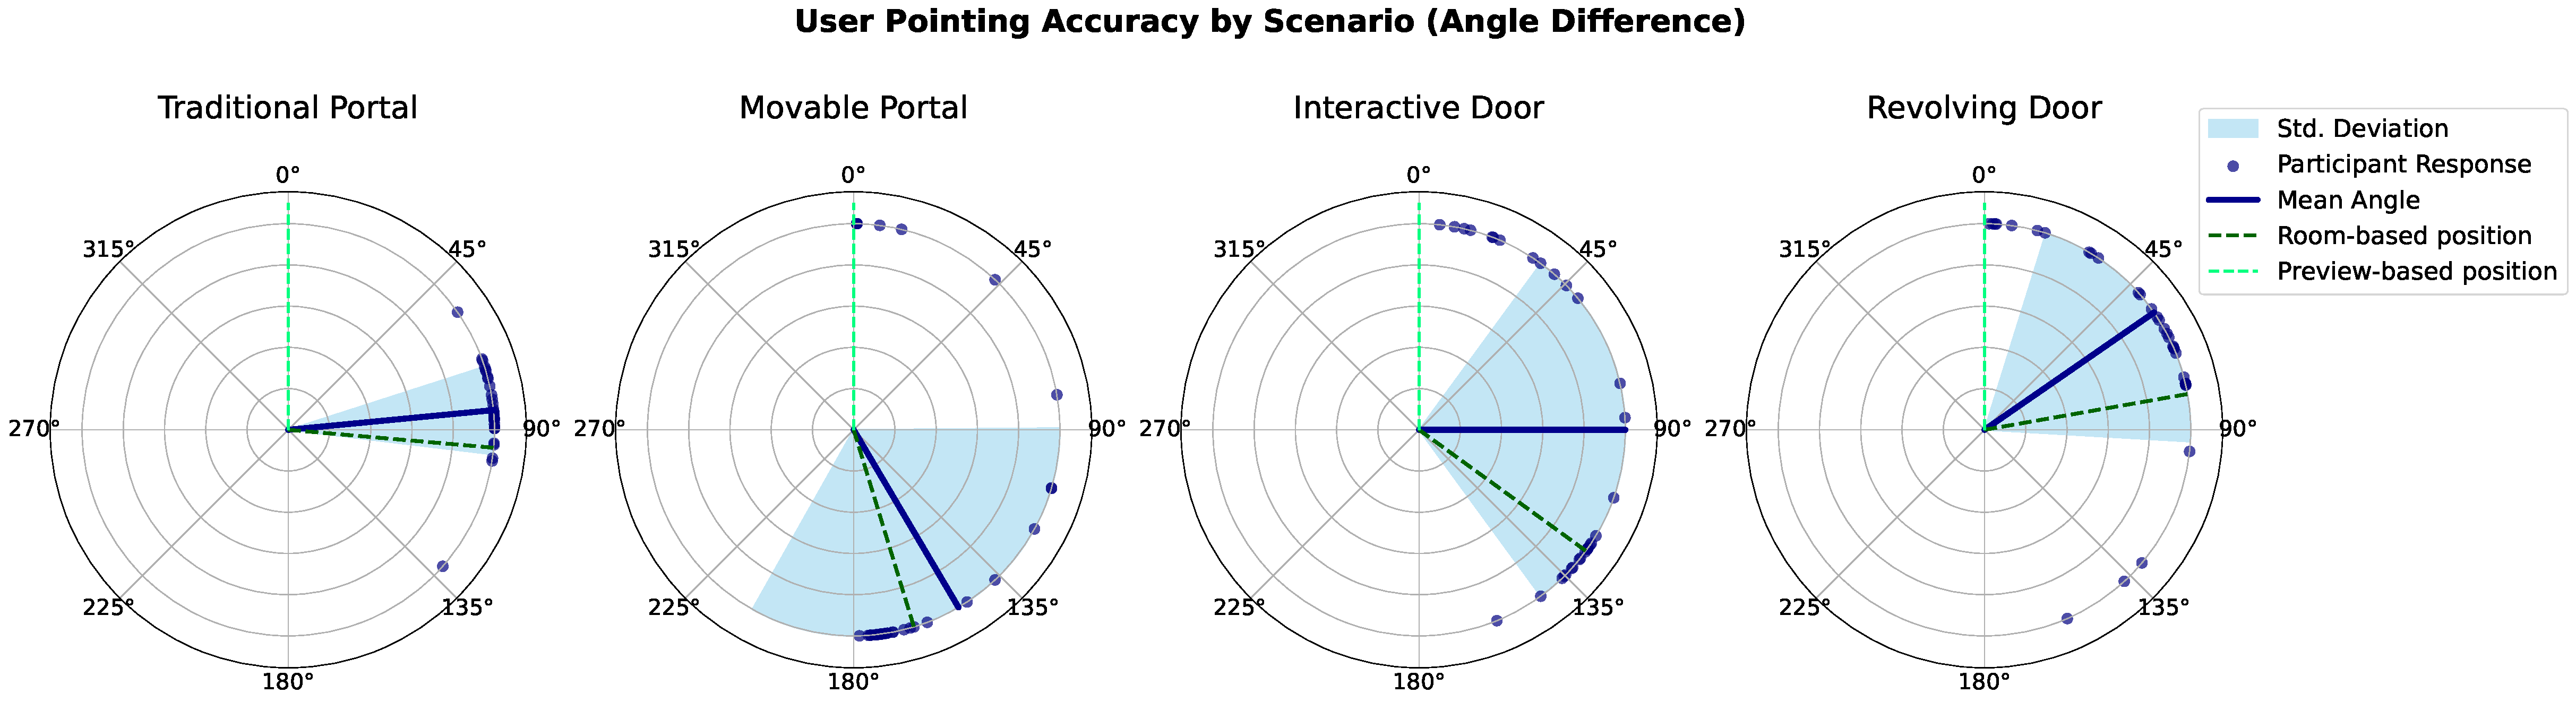
\includegraphics[width=\textwidth]{NOVAthesisFiles/Images/graphs/angle_difference_plot_with_stats.pdf}
    \caption[Polar plots of the distribution of angular error in the pointing task by portal condition.]
    {Polar plots showing the distribution of angular error in the pointing task by portal condition.}
    \label{fig:angle_plot}
\end{figure}

\subsection{Usability and Naturalness}
\label{sec:usability-naturalness}

To assess subjective user experience, at the end of each section, participants rated their agreement with two statements on a 7-point Likert 
scale (1=Strongly Disagree, 7=Strongly Agree): (1) “I found the transition between rooms natural” and 
(2) "I found the transition between rooms intuitive / easy to use". 


This data was analysed using a non-parametric Friedman test. Significant results were followed by post-hoc Wilcoxon signed-rank tests with a Bonferroni 
correction applied, resulting in a significance level of p $<$ .0083.

\textbf{Naturalness}: The user ratings for perceived naturalness are visualized in \autoref{fig:naturalness_results}. 
A Friedman test revealed a highly significant difference in perceived naturalness across the four portal types, $\chi$²(3, N=31) = 27.18, 
p $<$ .001. Post-hoc analysis showed that the Traditional Portal (M=5.61, SD=1.15) was rated as significantly more natural than both the 
Movable Portal (M=3.81, SD=1.66; p $<$ .001) and the Revolving Door Portal (M=4.35, SD=1.45; p $<$ .001). Additionally, 
the Interactive Door Portal (M=5.13, SD=1.38) was rated as significantly more natural than the Movable Portal (p = .0002).

\begin{figure}[t]
\centering
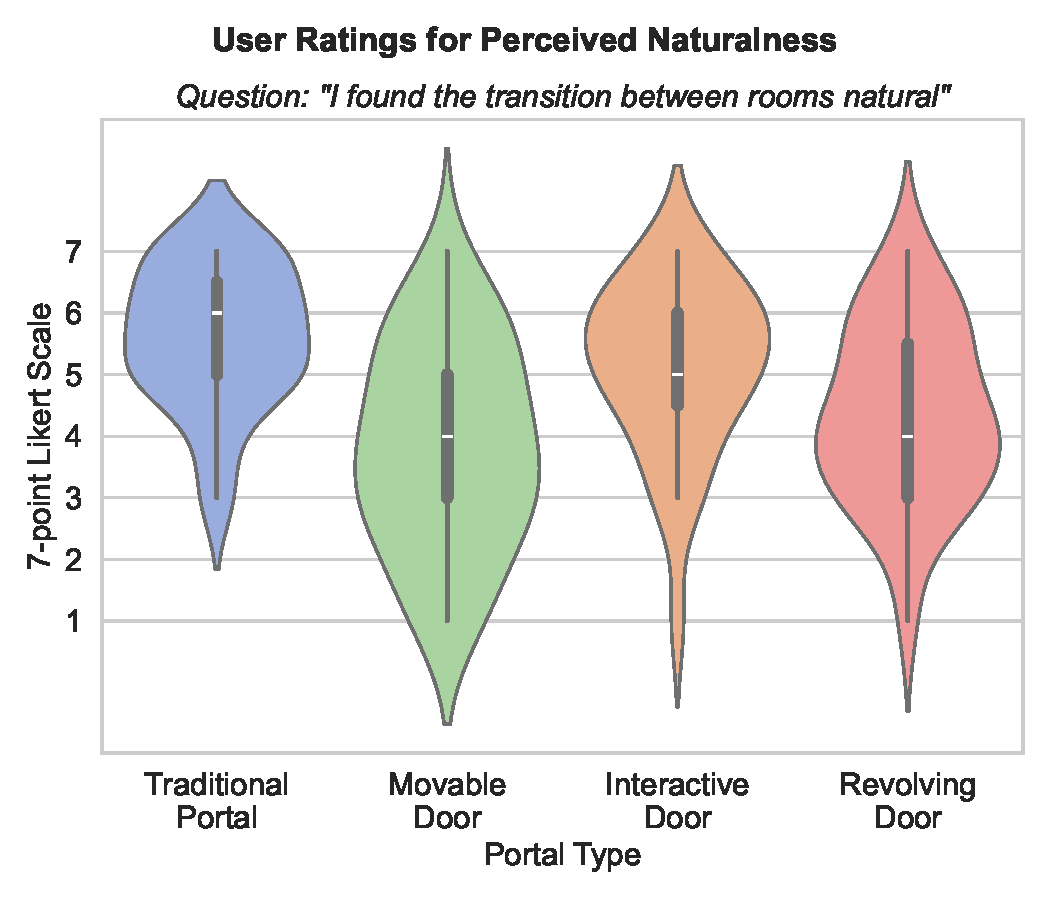
\includegraphics[width=.6\linewidth]{NOVAthesisFiles/Images/graphs/naturalness_violin_plot.pdf}
\caption{User ratings for Perceived Naturalness.}
\label{fig:naturalness_results}
\end{figure}

\begin{figure}[t]
\centering
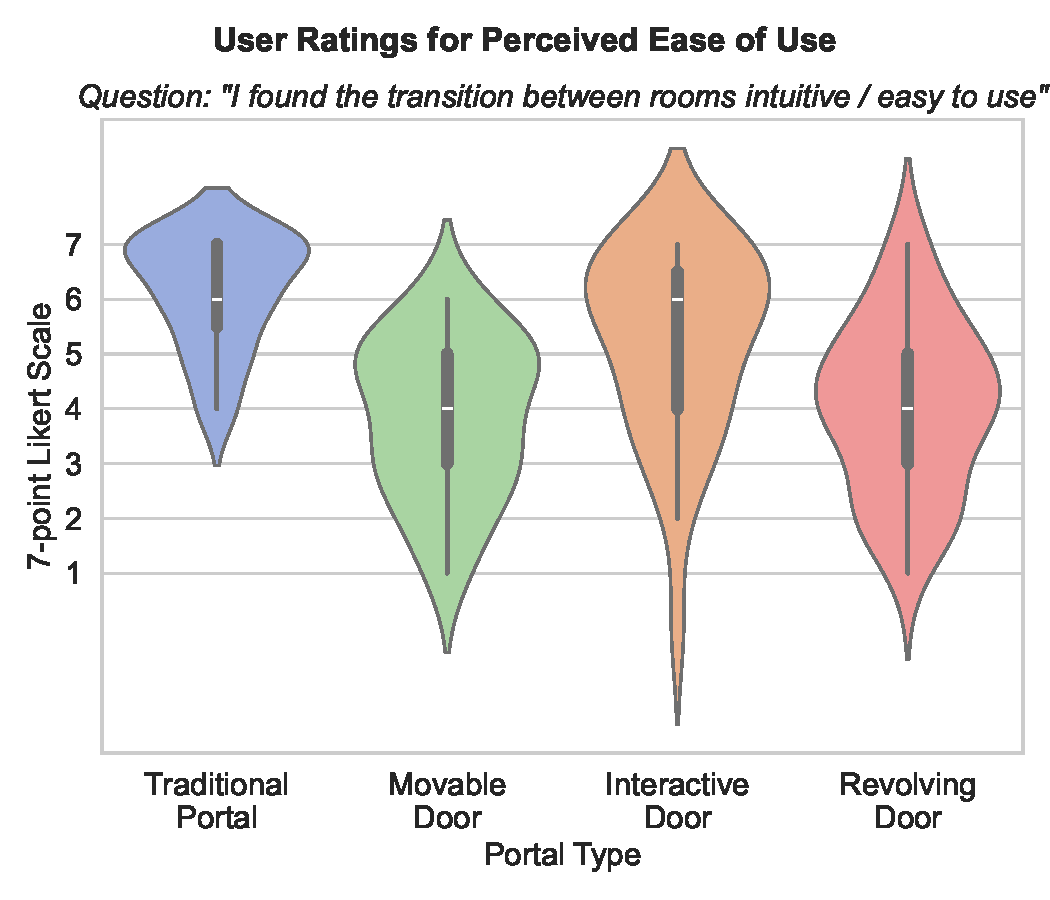
\includegraphics[width=.6\linewidth]{NOVAthesisFiles/Images/graphs/ease_of_use_violin_plot.pdf}
\caption{User ratings for Perceived Ease-of-Use.}
\label{fig:ease_of_use_results}
\end{figure}

\textbf{Ease of Use / Intuitiveness:} We found a highly significant effect of the portal type on perceived ease of use, 
$\chi$²(3, N=31) = 40.60, p $<$ .001, with results shown in \autoref{fig:ease_of_use_results}. Post-hoc tests revealed a 
clear hierarchy of usability. The Traditional Portal (M=6.13, SD=1.02) was rated as significantly easier to use than all 
other techniques: Interactive Door (M=5.19, SD=1.74; p = .0013), Revolving Door (M=4.03, SD=1.56; p $<$ .001), and 
Movable Portal (M=3.84, SD=1.44; p $<$ .001). Furthermore, the Interactive Door Portal was also rated as significantly easier 
to use than both the Revolving Door (p = .0054) and the Movable Portal (p = .0011). No significant difference was found between 
the Movable and Revolving Door portals, placing them together in the lowest tier for ease of use.


To complement the subjective ratings, we analysed objective usability issues recorded by the experimenter. 
The number of spoken hesitations (e.g., verbal expressions of confusion) and action-based tries 
($e.g.$, incorrect or repeated attempts to use a portal) for each participant were quantified.

A Friedman test confirmed that the differences between portal types were highly significant for both spoken hesitations 
($\chi$²(3, N=31) = 23.09, p $<$ .001) and action-based tries ($\chi$²(3, N=31) = 71.12, p $<$ .001). As in \autoref{fig:hesitations_plot}, 
the Revolving Door and Movable Portal generated a substantial number of usability issues. The Revolving Door, while producing a moderate 
number of spoken hesitations (M = 2.03), was associated with a higher mean of action-based tries (M = 13.48). The Movable Portal also 
proved challenging, resulting in the highest mean for spoken hesitations (M = 2.39) and a high number of action-based tries (M = 8.61). 
In contrast, the Interactive Door (Hesitations: M = 0.45, Tries: M = 1.39) and especially the Traditional Portal (Hesitations: M = 0.35, 
Tries: M = 0.19) were associated with negligible usability problems.

\begin{figure}[t]
\centering
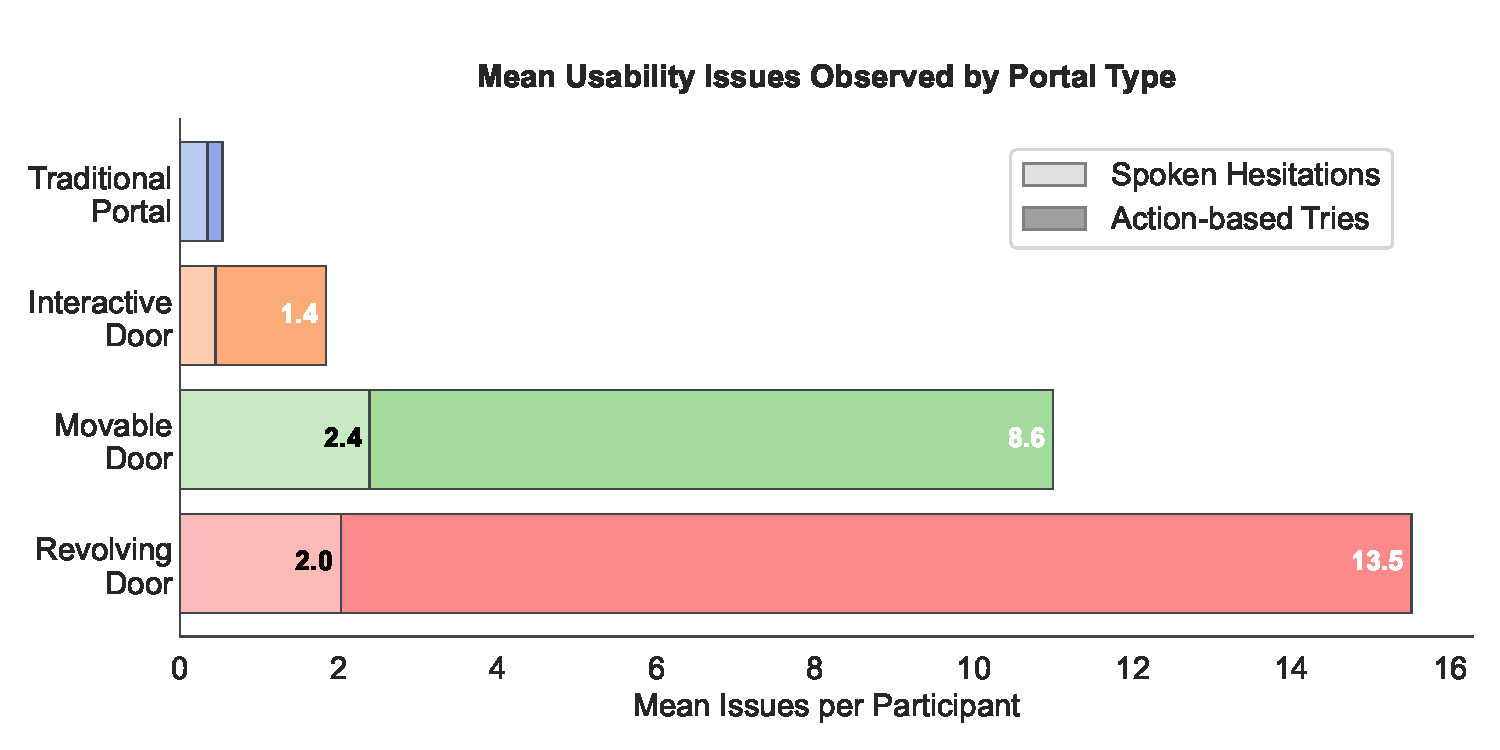
\includegraphics[width=.8\textwidth]{NOVAthesisFiles/Images/graphs/hesitations_stacked_horizontal_plot.pdf}
\caption{Mean number of usability issues per participant by portal type. The stacked horizontal bars show spoken hesitations (light tone) and action-based tries (bright tone) for each portal type.}
\label{fig:hesitations_plot}
\end{figure}


\subsection{User Preference}

To assess overall preferences, participants ranked the four portal techniques on a scale from 1 (most preferred) to 4 (least preferred) 
on the post-session questionnaire. An initial Friedman test, $\chi$²(3, N=30)= 70.67, p$<$0.001, shows a statistically significant 
difference in user preference between the four locomotion techniques, indicating that participants did not rank all techniques equally. 
\autoref{fig:user-preference} shows the results of the preference rankings. Traditional Portals scored the highest, followed by the 
Interactive Doors, then Revolving Doors, with Movable Portals being ranked the lowest. 

Adjacent comparisons were conducted within each rank based on technique frequency, with only one reaching statistical significance: 
at the 4th rank, Revolving Doors were significantly more likely to be rated least preferred compared to Interactive Doors 
(p = 0.0153 after Bonferroni correction). Although participants showed a clear preference towards Traditional Portals, this 
preference missed statistical significance when compared to the Interactive Doors(p = 0.0169 vs adjusted $\alpha$ = 0.0167), 
the second most top-ranked technique.

\begin{figure}[h]
    \centering
    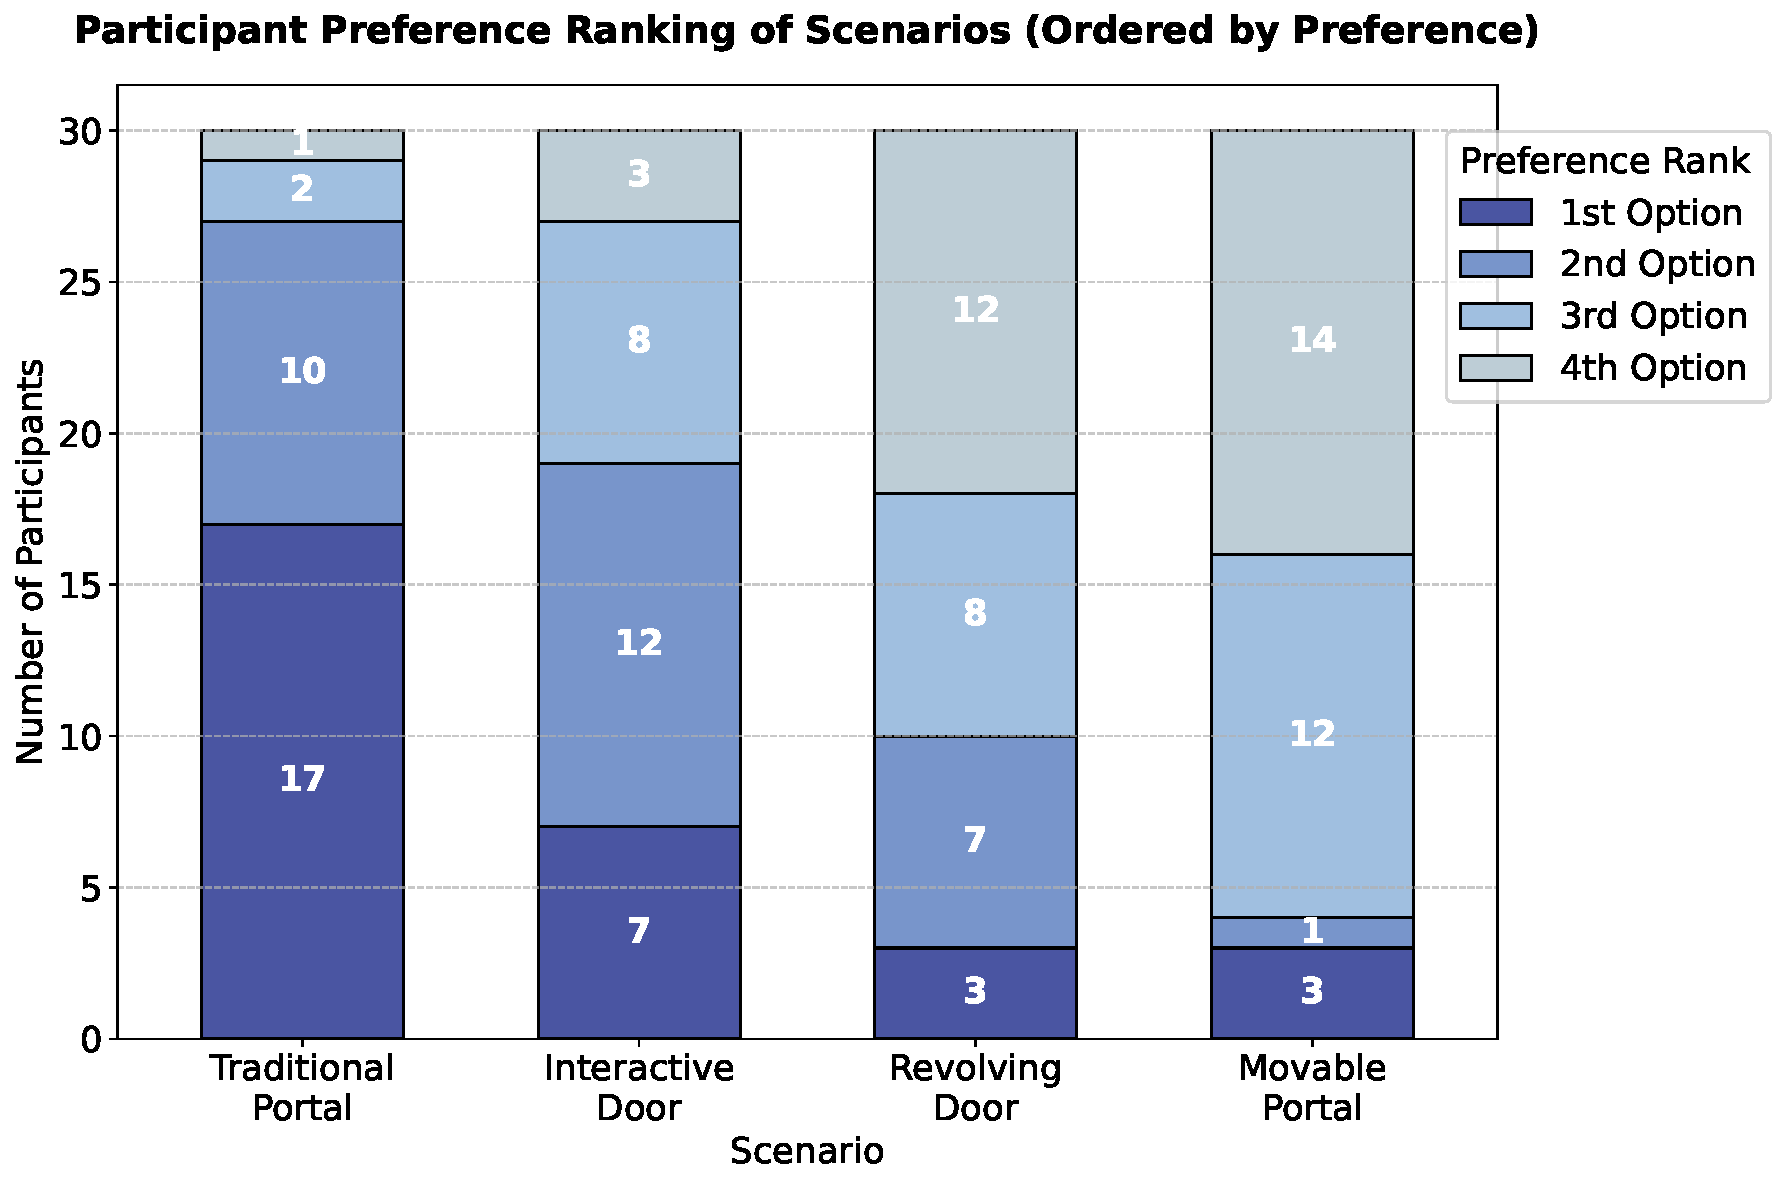
\includegraphics[width=.65\textwidth]{NOVAthesisFiles/Images/graphs/scenario_preference_plot.pdf}
    \caption[Participants preference rankings over portal techniques.]
    {Participant preference rankings for the four interaction scenarios.}
    \label{fig:user-preference}
\end{figure}

\subsection{Presence}
\label{sec:presence}

As previously mentioned, presence was measured using the Igroup Presence Questionnaire (IPQ). 
Overall, participants reported moderate to high scores across subscales (Spatial Presence: M~=~5.5, SD~=~0.45; 
Involvement: M~=~4.42, SD~=~0.4; Experienced Realism: M~=~4.58, SD~=~0.78), indicating a moderate to high sense of 
presence during the \gls{VR} experience. 

\subsection{Cybersickness}
\label{sec:cybersickness}
Cybersickness was assessed using the Virtual Reality Sickness Questionnaire (VRSQ). 
Participants reported low levels of symptoms both before (M~=~2.23, SD~=~3.13) and after the session (M~=~2.68, SD~=~3.91),
suggesting that the experience had minimal impact on cybersickness.

\todo{algo mais a se dizer? talvez juntar com o presence?}

\subsection{Qualitative Feedback}

Participants explained their preferences for the different portal types through 
open-ended questions in the post-session questionnaire. We also collected voluntary oral commentary provided throughout the session.

During the Traditional Portal section, participants expressed some dissatisfaction with having to walk around the portals to preview 
the next room before entering. Concerns were also raised about getting lost or forgetting which rooms they had already visited. 
Despite these issues, most participants justified their preference for Traditional Portals by describing them as "the easiest to use" 
and "most natural". Several participants noted that this technique provided the closest experience to a real museum, as "in a real museum, 
you only have to pass through a doorway to move to the next room".

Regarding the Movable Portal, some participants reported feelings of confusion (e.g., "What am I supposed to do?", "Did I do that?") 
or discomfort (e.g., "This feels weird.", "Don't spin!"(speaking to the portal)), while others expressed amusement and enjoyment 
(e.g., "This is fun!", "I can move it? How cool!"). Participants that preferred this technique overall
appreciated the sense of control from being able to move the portal. The steep learning curve and higher effort required were frequently 
cited drawbacks.

Participants reacted positively to the Interactive Door upon first contact (e.g., "This one is cool!", "Ah, wow!"). 
Questionnaire responses highlighted that the door's opening mechanism felt intuitive and immersive, which participants often attributed 
to its resemblance to real-world door interaction, requiring minimal cognitive effort. A few participants did report some initial 
confusion regarding the portal's movement, noting that it follows the door as it is opened.

Initial interactions with the Revolving Door were challenging, with participants asking questions such as "Am I supposed to pull 
it or push it?" and "I was seeing where I was going... but now I don't?" or expressing general confusion (e.g., "This is weird."). 
However, by the end of the session, participants reported greater comfort with the technique (e.g., "After understanding it, it was easy.").
While the steep learning curve was frequently mentioned as a drawback in the questionnaire, several participants who preferred the Revolving
Door highlighted its fun and immersive qualities.

\section{Discussion}
\label{sec:discussion}

The main goal of the presented work was to evaluate four \gls{VR} locomotion techniques based on natural walking with portals, 
focusing on their impact on usability, spatial understanding, and user preference. The findings from the study with 31 participants 
provided insights into these aspects of \gls{UX}, allowing the purpose of this study to be addressed by tackling the research questions 
defined in Section~\ref{sec:objectives-and-researh-questions}.

In this section, the research questions are addressed through the presentation and discussion of the insights gained from the user study.

\todo{Estas perguntas deviam ser mini-títulos como na tese da Rita}
\textbf{Q1 - What are the effects of a dynamic preview in regard to users' sense of space?}

The pointing task, performed at the end of every section of the virtual museum, was designed to address this issue, by providing a better 
insight into how the participants perceived space. The results reveal nuanced differences in how each portal design affects the perception 
users have of the layout of the \gls{VE}, but highlights a big difference between Traditional Portals and the other variant portal designs.

The results of the pointing task in the Traditional Portal section present the lowest variation in angular error, with most responses 
clustering around a median of 85.62\textdegree. This angle closely corresponds to the position of the object in the overlapping 
architecture. In contrast, responses for the other techniques were more widely dispersed, as answers no longer clustered on the same 
position. Several participants utilized the preview capabilities of the portal variants when prompted to point towards the object, pointing 
at the object through the portal's preview. 

The clear distinction between the results of the portal variants' sections and the Traditional Portal's section suggests that participants 
relied on the preview features to inform their spatial judgments, indicating that dynamic previews can influence and potentially enhance 
the sense of spatial continuity.


\textbf{Q2 - What elements of \gls{UX} do users prioritize when interacting with these navigation techniques?}

The results of the study suggest that participants primarily prioritized ease of use and naturalness when interacting with the different 
portal designs. The preference rankings reveal that a majority of participants preferred to use the Traditional Portals and the 
Interactive Portals, followed by the Revolving Door and the Movable Portal.

Traditional Portals were consistently rated as the most intuitive and easiest to use, which corresponds with the low amount of usability 
issues registered when using this portal and the commentary provided by the participants. Interactive Doors were also perceived 
positively, as their mechanics closely mimicked real-world door interactions, making the transition feel natural and intuitive, also 
backed by the low number of usability issues and participant commentary. 
In contrast, Movable Portals and Revolving Doors, while appreciated by some participants for the added sense of control or the stronger 
perception of continuous space they provided, were generally hindered by steeper learning curves and higher cognitive demands. 

Taken together, these findings indicate that users tend to value straightforward, familiar, and low-effort interactions above more complex 
mechanics that may enhance spatial continuity but reduce immediate usability. 


\textbf{Q3 - What are the strong points for each of these techniques, in regard to \gls{VE} navigation?} 

Through the commentary and experience observed in this study, it was possible to conclude that each portal technique 
presented distinct strengths for \gls{VE} navigation. 

Traditional Portals stood out for their simplicity and reliability, being mostly praised for their ease of use and efficiency. 
Movable Portals offered participants a sense of control over their navigation, enabling them to reposition the portal and adjust 
how space was experienced, which some users found engaging and empowering despite the higher effort required. 
Interactive Doors were valued for their intuitive and immersive interaction, as the door-opening mechanic resembled a 
familiar real-world action and contributed to a natural sense of transition between rooms. 
Revolving Doors, while initially less intuitive, were highlighted for providing the smoothest feeling of spatial continuity, 
with their guided redirection enhancing the perception of flow across rooms once participants became accustomed to the technique.

\section{Summary}
\label{sec:summary}

\todo{Completar de acordo como ficar no final}

